\documentclass[../main.tex]{subfiles}
\begin{document}
\chapter{提案手法}

\section{提案}

本研究では、tkinterを用いてボールの動きを描画する手法を用いた.事前に全てのパスの通りにタグを付けておき,必要なパスの線のタグ名を入力することで
ボールの動きを描画した.
このツールを用いてボールの動きを描画することで,簡易的な操作を実現する.操作者は動画を読み込むこともなく,パスが通ったポジションを記録したメモに基づき
適切な数値とローマ字の組み合わせを入力することで,感覚的な操作が可能になる.

\section{基本仕様}

2章で述べた退水セットにおけるポジション番号以外に,本研究では7・8・9番のポジション番号を設定すると共に,ゴールをゴールキーパーから見て左からJ・K・Lと設定した.
これは,5・6番ポジションのオフェンス選手が斜めに切り上がることが多い3つのポジションを設定したものだ.また,ゴールを決められた・決めた際にどこにシュートが飛んで
来たのかということも重要になるため,本研究でのみ使用されるポジションを以下の図のように設定した.\ref{img:ExclusionNO}

\begin{figure}[ht]
    \begin{center}
        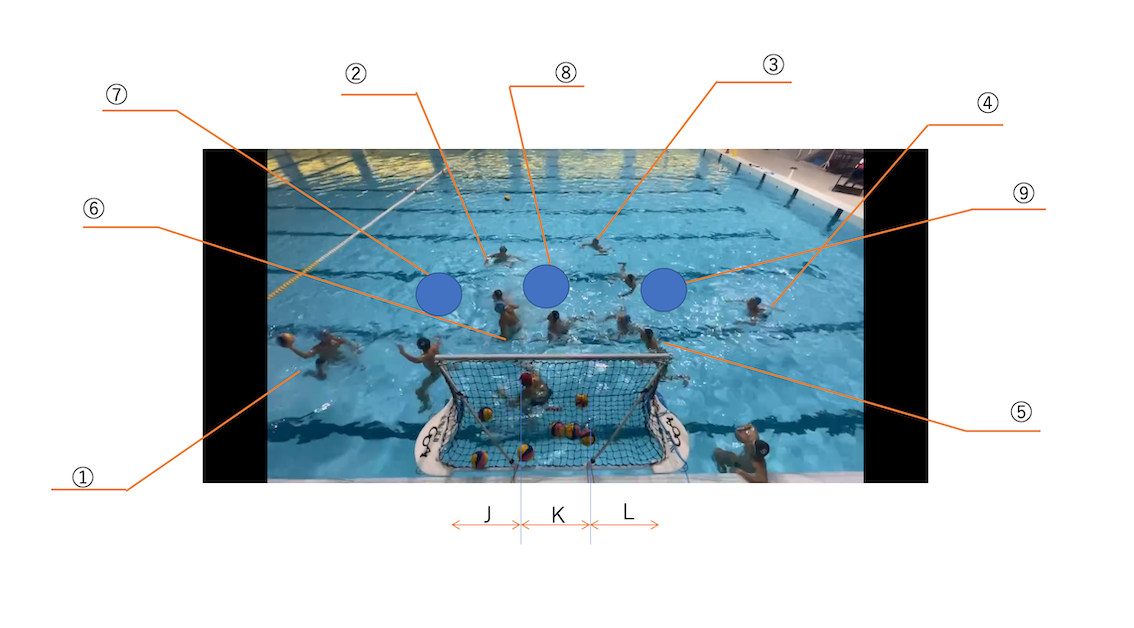
\includegraphics{img/02.png}
        \caption{退水セットでのポジション番号並びにゴールの分割方法}
        \label{img:ExclusionNO}
    \end{center}
\end{figure}



tkinter内でこの1番〜9番,JKLの12ヶ所に座標を設定する.前述のパスのタグとは,1番から2番にパスが通った場合には「12p」と操作画面に入力することで
操作者が座標を入力することなく座標間に線を引くことができるようにしたものである.例えば一度の退水セットでボールが1番・2番・3番・4番・5番のポジションに渡り
最終的にJの位置にゴールが決まった際には,メモには「12345j」という記載をした.その場合はツールの入力画面で
「12p」「23p」「34p」「45p」「5j」という値を適切な箇所に入力し,再生することで以下のような出力を得られる.\ref{img:ballmovement12345j}

\begin{figure}[ht]
    \begin{center}
        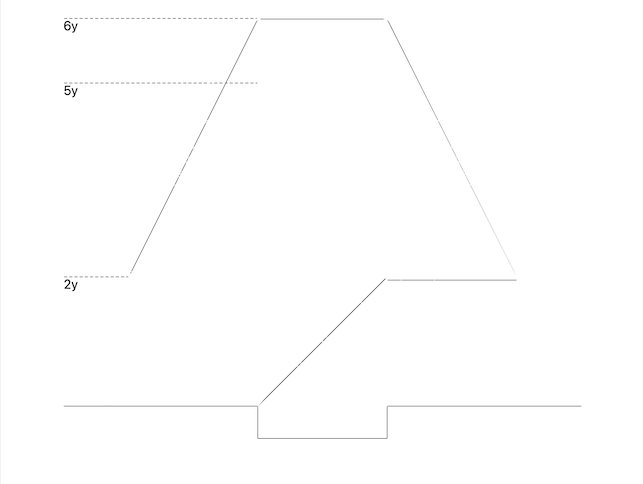
\includegraphics{img/05.png}
        \caption{ボールが12345jと動いた際の出力}
    \label{img:ballmovement12345j}
    \end{center}
\end{figure}

\end{document}